%--------------------
% Packages
% -------------------
\documentclass[11pt,english]{article}
\usepackage{amsfonts}
\usepackage[left=2.5cm,top=2cm,right=2.5cm,bottom=3cm,bindingoffset=0cm]{geometry}
\usepackage{amsmath, amsthm, amssymb}
\usepackage{tikz}
\usetikzlibrary{calc}
\usetikzlibrary{decorations.pathreplacing,calligraphy}
\usepackage{fancyhdr}
%\usepackage{currfile}
\usepackage{nicefrac}
\usepackage{cite}
\usepackage{graphicx}
\usepackage{caption}
\usepackage{longtable}
\usepackage{rotating}
\usepackage{lscape}
\usepackage{booktabs}
\usepackage{float}
\usepackage{placeins}
\usepackage{setspace}
\usepackage[font=itshape]{quoting}
\onehalfspacing
\usepackage{mathrsfs}
\usepackage{tcolorbox}
\usepackage{xcolor}
\usepackage{subcaption}
\usepackage{float}
\usepackage[multiple]{footmisc}
\usepackage[T1]{fontenc}
\usepackage[sc]{mathpazo}
\usepackage{listings}
\usepackage{longtable}
\definecolor{cmured}{RGB}{175,30,45}
\definecolor{macroblue}{RGB}{56,108,176}
\usepackage[format=plain,
            labelfont=bf,
            textfont=]{caption}
\usepackage[colorlinks=true,citecolor=macroblue,linkcolor=macroblue,urlcolor=macroblue]{hyperref}
\usepackage{varioref}
\usepackage{chngcntr}
\usepackage{datetime}

\definecolor{darkgreen}{RGB}{30,175,88}
\definecolor{darkblue}{RGB}{30,118,175}
\definecolor{maroon}{rgb}{0.66,0,0}
\definecolor{darkgreen}{rgb}{0,0.69,0}

%Counters
\newtheorem{theorem}{Theorem}[section] 
\newtheorem{proposition}{Proposition}
\newtheorem{lemma}{Lemma}
\newtheorem{corollary}{Corollary}
\newtheorem{assumption}{Assumption}
\newtheorem{axiom}{Axiom}
\newtheorem{case}{Case}
\newtheorem{claim}{Claim}
\newtheorem{condition}{Condition}
\newtheorem{definition}{Definition}
\newtheorem{example}{Example}
\newtheorem{notation}{Notation}
\newtheorem{remark}{Remark}


\hypersetup{ 	
pdfsubject = {},
pdftitle = {TidyTuesday Week 39},
pdfauthor = {Pranay Gundam},
linkcolor= macroblue
}


\title{\textbf{TidyTuesday Week 39}}
\author{Pranay Gundam}


%-----------------------
% Begin document
%-----------------------
\begin{document}

\maketitle

\tableofcontents

\section{Weekly Summary}


\section{Date: 2024-09-23}
\noindent \textbf{Series ID: ACOILWTICO} 

\noindent This series is titled Crude Oil Prices: West Texas Intermediate (WTI) - Cushing, Oklahoma and has a frequency of Annual. The units are Dollars per Barrel and the seasonal adjustment is Not Seasonally Adjusted.The observation start date is 1986-01-01 and the observation end date is 2023-01-01.The popularity of this series is 22. \\ 

\noindent \textbf{Series ID: STTMINWGNY} 

\noindent This series is titled State Minimum Wage Rate for New York and has a frequency of Annual. The units are Dollars per Hour and the seasonal adjustment is Not Seasonally Adjusted.The observation start date is 1968-01-01 and the observation end date is 2024-01-01.The popularity of this series is 37. \\ 

\subsection{Regression Tables and Plots}
\begin{center}
\begin{tabular}{lclc}
\toprule
\textbf{Dep. Variable:}          & value\_fred\_STTMINWGNY & \textbf{  R-squared:         } &     0.444   \\
\textbf{Model:}                  &           OLS           & \textbf{  Adj. R-squared:    } &     0.428   \\
\textbf{Method:}                 &      Least Squares      & \textbf{  F-statistic:       } &     28.74   \\
\textbf{Date:}                   &     Mon, 23 Sep 2024    & \textbf{  Prob (F-statistic):} &  4.97e-06   \\
\textbf{Time:}                   &         13:31:51        & \textbf{  Log-Likelihood:    } &   -84.492   \\
\textbf{No. Observations:}       &              38         & \textbf{  AIC:               } &     173.0   \\
\textbf{Df Residuals:}           &              36         & \textbf{  BIC:               } &     176.3   \\
\textbf{Df Model:}               &               1         & \textbf{                     } &             \\
\textbf{Covariance Type:}        &        nonrobust        & \textbf{                     } &             \\
\bottomrule
\end{tabular}
\begin{tabular}{lcccccc}
                                 & \textbf{coef} & \textbf{std err} & \textbf{t} & \textbf{P$> |$t$|$} & \textbf{[0.025} & \textbf{0.975]}  \\
\midrule
\textbf{const}                   &       3.3324  &        0.716     &     4.652  &         0.000        &        1.880    &        4.785     \\
\textbf{value\_fred\_ACOILWTICO} &       0.0699  &        0.013     &     5.361  &         0.000        &        0.043    &        0.096     \\
\bottomrule
\end{tabular}
\begin{tabular}{lclc}
\textbf{Omnibus:}       &  8.225 & \textbf{  Durbin-Watson:     } &    0.249  \\
\textbf{Prob(Omnibus):} &  0.016 & \textbf{  Jarque-Bera (JB):  } &    7.567  \\
\textbf{Skew:}          &  1.082 & \textbf{  Prob(JB):          } &   0.0227  \\
\textbf{Kurtosis:}      &  3.309 & \textbf{  Cond. No.          } &     106.  \\
\bottomrule
\end{tabular}
%\caption{OLS Regression Results}
\end{center}

Notes: \newline
 [1] Standard Errors assume that the covariance matrix of the errors is correctly specified.

\begin{figure}
\centering
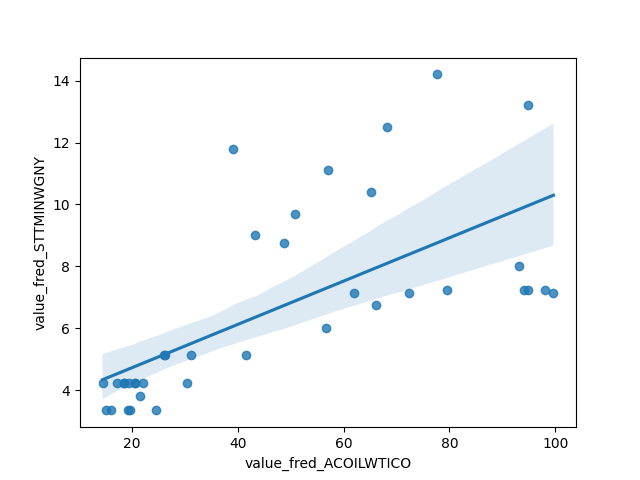
\includegraphics[scale = 0.9]{plots/plot_2024-09-23.png}
\caption{Regression Plot for 2024-09-23}
\end{figure}
\newpage


\section{Date: 2024-09-24}
\noindent \textbf{Series ID: CEU9000000010} 

\noindent This series is titled Women Employees, Government and has a frequency of Monthly. The units are Thousands of Persons and the seasonal adjustment is Not Seasonally Adjusted.The observation start date is 1964-01-01 and the observation end date is 2024-08-01.The popularity of this series is 1. \\ 

\noindent \textbf{Series ID: DLTRUCKSNSA} 

\noindent This series is titled Motor Vehicle Retail Sales: Domestic Light Weight Trucks and has a frequency of Monthly. The units are Thousands of Units and the seasonal adjustment is Not Seasonally Adjusted.The observation start date is 1967-01-01 and the observation end date is 2024-08-01.The popularity of this series is 4. \\ 

\subsection{Regression Tables and Plots}
\begin{center}
\begin{tabular}{lclc}
\toprule
\textbf{Dep. Variable:}             & value\_fred\_DLTRUCKSNSA & \textbf{  R-squared:         } &     0.747   \\
\textbf{Model:}                     &           OLS            & \textbf{  Adj. R-squared:    } &     0.747   \\
\textbf{Method:}                    &      Least Squares       & \textbf{  F-statistic:       } &     2038.   \\
\textbf{Date:}                      &     Tue, 24 Sep 2024     & \textbf{  Prob (F-statistic):} & 3.71e-208   \\
\textbf{Time:}                      &         22:43:06         & \textbf{  Log-Likelihood:    } &   -4259.9   \\
\textbf{No. Observations:}          &             692          & \textbf{  AIC:               } &     8524.   \\
\textbf{Df Residuals:}              &             690          & \textbf{  BIC:               } &     8533.   \\
\textbf{Df Model:}                  &               1          & \textbf{                     } &             \\
\textbf{Covariance Type:}           &        nonrobust         & \textbf{                     } &             \\
\bottomrule
\end{tabular}
\begin{tabular}{lcccccc}
                                    & \textbf{coef} & \textbf{std err} & \textbf{t} & \textbf{P$> |$t$|$} & \textbf{[0.025} & \textbf{0.975]}  \\
\midrule
\textbf{const}                      &    -297.4786  &       16.845     &   -17.660  &         0.000        &     -330.552    &     -264.406     \\
\textbf{value\_fred\_CEU9000000010} &       0.0728  &        0.002     &    45.147  &         0.000        &        0.070    &        0.076     \\
\bottomrule
\end{tabular}
\begin{tabular}{lclc}
\textbf{Omnibus:}       & 20.866 & \textbf{  Durbin-Watson:     } &    0.443  \\
\textbf{Prob(Omnibus):} &  0.000 & \textbf{  Jarque-Bera (JB):  } &   33.310  \\
\textbf{Skew:}          & -0.239 & \textbf{  Prob(JB):          } & 5.85e-08  \\
\textbf{Kurtosis:}      &  3.963 & \textbf{  Cond. No.          } & 4.05e+04  \\
\bottomrule
\end{tabular}
%\caption{OLS Regression Results}
\end{center}

Notes: \newline
 [1] Standard Errors assume that the covariance matrix of the errors is correctly specified. \newline
 [2] The condition number is large, 4.05e+04. This might indicate that there are \newline
 strong multicollinearity or other numerical problems.

\begin{figure}
\centering
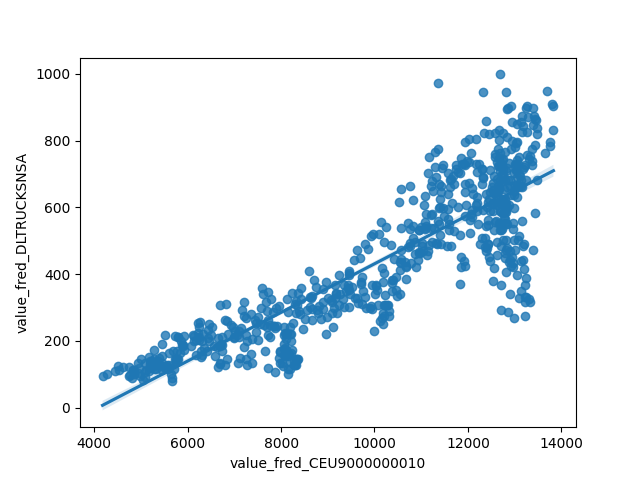
\includegraphics[scale = 0.9]{plots/plot_2024-09-24.png}
\caption{Regression Plot for 2024-09-24}
\end{figure}
\newpage


\section{Date: 2024-09-25}
\noindent \textbf{Series ID: NPPGPL2} 

\noindent This series is titled Nonfarm Private Goods - Producing Large Payroll Employment (1000+) (DISCONTINUED) and has a frequency of Monthly. The units are Thousands and the seasonal adjustment is Seasonally Adjusted.The observation start date is 2005-01-01 and the observation end date is 2022-05-01.The popularity of this series is 1. \\ 

\noindent \textbf{Series ID: MDOTHFRA} 

\noindent This series is titled Mortgage Debt Outstanding by Type of Holder: Federal and Related Agencies (DISCONTINUED) and has a frequency of Quarterly, End of Period. The units are Millions of Dollars and the seasonal adjustment is Not Seasonally Adjusted.The observation start date is 1949-01-01 and the observation end date is 2019-07-01.The popularity of this series is 3. \\ 

\subsection{Regression Tables and Plots}
\begin{center}
\begin{tabular}{lclc}
\toprule
\textbf{Dep. Variable:}       & value\_fred\_MDOTHFRA & \textbf{  R-squared:         } &     0.350   \\
\textbf{Model:}               &          OLS          & \textbf{  Adj. R-squared:    } &     0.339   \\
\textbf{Method:}              &     Least Squares     & \textbf{  F-statistic:       } &     30.71   \\
\textbf{Date:}                &    Wed, 25 Sep 2024   & \textbf{  Prob (F-statistic):} &  7.98e-07   \\
\textbf{Time:}                &        10:06:53       & \textbf{  Log-Likelihood:    } &   -929.62   \\
\textbf{No. Observations:}    &             59        & \textbf{  AIC:               } &     1863.   \\
\textbf{Df Residuals:}        &             57        & \textbf{  BIC:               } &     1867.   \\
\textbf{Df Model:}            &              1        & \textbf{                     } &             \\
\textbf{Covariance Type:}     &       nonrobust       & \textbf{                     } &             \\
\bottomrule
\end{tabular}
\begin{tabular}{lcccccc}
                              & \textbf{coef} & \textbf{std err} & \textbf{t} & \textbf{P$> |$t$|$} & \textbf{[0.025} & \textbf{0.975]}  \\
\midrule
\textbf{const}                &    2.218e+07  &     3.35e+06     &     6.616  &         0.000        &     1.55e+07    &     2.89e+07     \\
\textbf{value\_fred\_NPPGPL2} &   -2599.1459  &      468.991     &    -5.542  &         0.000        &    -3538.285    &    -1660.007     \\
\bottomrule
\end{tabular}
\begin{tabular}{lclc}
\textbf{Omnibus:}       &  6.887 & \textbf{  Durbin-Watson:     } &    0.116  \\
\textbf{Prob(Omnibus):} &  0.032 & \textbf{  Jarque-Bera (JB):  } &    6.256  \\
\textbf{Skew:}          & -0.782 & \textbf{  Prob(JB):          } &   0.0438  \\
\textbf{Kurtosis:}      &  3.312 & \textbf{  Cond. No.          } & 1.07e+05  \\
\bottomrule
\end{tabular}
%\caption{OLS Regression Results}
\end{center}

Notes: \newline
 [1] Standard Errors assume that the covariance matrix of the errors is correctly specified. \newline
 [2] The condition number is large, 1.07e+05. This might indicate that there are \newline
 strong multicollinearity or other numerical problems.

\begin{figure}
\centering
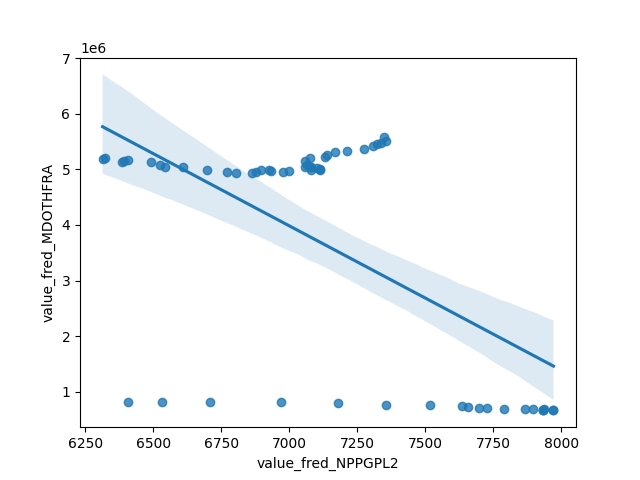
\includegraphics[scale = 0.9]{plots/plot_2024-09-25.png}
\caption{Regression Plot for 2024-09-25}
\end{figure}
\newpage


\section{Date: 2024-09-26}
\noindent \textbf{Series ID: MESTFININSRGSP} 

\noindent This series is titled Real Gross Domestic Product: Finance and Insurance (52) in the Mideast BEA Region and has a frequency of Annual. The units are Millions of Chained 2017 Dollars and the seasonal adjustment is Not Seasonally Adjusted.The observation start date is 1997-01-01 and the observation end date is 2023-01-01.The popularity of this series is 1. \\ 

\noindent \textbf{Series ID: W514RC1A027NBEA} 

\noindent This series is titled Government current receipts: Excluding imputations and has a frequency of Annual. The units are Billions of Dollars and the seasonal adjustment is Not Seasonally Adjusted.The observation start date is 1929-01-01 and the observation end date is 2022-01-01.The popularity of this series is 1. \\ 

\subsection{\subsection{Regression Tables and Plots}}
\begin{center}
\begin{tabular}{lclc}
\toprule
\textbf{Dep. Variable:}              & value\_fred\_W514RC1A027NBEA & \textbf{  R-squared:         } &     0.606   \\
\textbf{Model:}                      &             OLS              & \textbf{  Adj. R-squared:    } &     0.589   \\
\textbf{Method:}                     &        Least Squares         & \textbf{  F-statistic:       } &     36.87   \\
\textbf{Date:}                       &       Thu, 26 Sep 2024       & \textbf{  Prob (F-statistic):} &  2.86e-06   \\
\textbf{Time:}                       &           12:14:24           & \textbf{  Log-Likelihood:    } &   -211.35   \\
\textbf{No. Observations:}           &                26            & \textbf{  AIC:               } &     426.7   \\
\textbf{Df Residuals:}               &                24            & \textbf{  BIC:               } &     429.2   \\
\textbf{Df Model:}                   &                 1            & \textbf{                     } &             \\
\textbf{Covariance Type:}            &          nonrobust           & \textbf{                     } &             \\
\bottomrule
\end{tabular}
\begin{tabular}{lcccccc}
                                     & \textbf{coef} & \textbf{std err} & \textbf{t} & \textbf{P$> |$t$|$} & \textbf{[0.025} & \textbf{0.975]}  \\
\midrule
\textbf{const}                       &   -3061.1692  &     1234.241     &    -2.480  &         0.021        &    -5608.518    &     -513.820     \\
\textbf{value\_fred\_MESTFININSRGSP} &       0.0183  &        0.003     &     6.072  &         0.000        &        0.012    &        0.024     \\
\bottomrule
\end{tabular}
\begin{tabular}{lclc}
\textbf{Omnibus:}       &  3.731 & \textbf{  Durbin-Watson:     } &    0.868  \\
\textbf{Prob(Omnibus):} &  0.155 & \textbf{  Jarque-Bera (JB):  } &    2.374  \\
\textbf{Skew:}          &  0.721 & \textbf{  Prob(JB):          } &    0.305  \\
\textbf{Kurtosis:}      &  3.332 & \textbf{  Cond. No.          } & 3.02e+06  \\
\bottomrule
\end{tabular}
%\caption{OLS Regression Results}
\end{center}

Notes: \newline
 [1] Standard Errors assume that the covariance matrix of the errors is correctly specified. \newline
 [2] The condition number is large, 3.02e+06. This might indicate that there are \newline
 strong multicollinearity or other numerical problems.

\begin{figure}
\centering
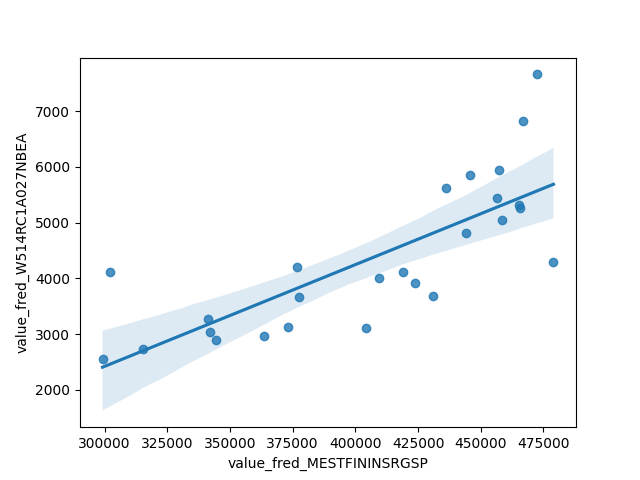
\includegraphics[scale = 0.9]{plots/plot_2024-09-26.png}
\caption{Regression Plot for 2024-09-26}
\end{figure}
\newpage


\include{tex_things/day_2024-09-27}

\section{Date: 2024-09-28}
\noindent \textbf{Series ID: PECILBU18MA25023A647NCEN} 

\noindent This series is titled 90% Confidence Interval Lower Bound of Estimate of People Age 0-17 in Poverty for Plymouth County, MA and has a frequency of Annual. The units are Persons and the seasonal adjustment is Not Seasonally Adjusted.The observation start date is 1989-01-01 and the observation end date is 2022-01-01.The popularity of this series is 1. \\ 

\noindent \textbf{Series ID: DLTRUCKSNSA} 

\noindent This series is titled Motor Vehicle Retail Sales: Domestic Light Weight Trucks and has a frequency of Monthly. The units are Thousands of Units and the seasonal adjustment is Not Seasonally Adjusted.The observation start date is 1967-01-01 and the observation end date is 2024-08-01.The popularity of this series is 4. \\ 

\subsection{\subsection{Regression Tables and Plots}}
\begin{center}
\begin{tabular}{lclc}
\toprule
\textbf{Dep. Variable:}                        & value\_fred\_DLTRUCKSNSA & \textbf{  R-squared:         } &     0.354   \\
\textbf{Model:}                                &           OLS            & \textbf{  Adj. R-squared:    } &     0.330   \\
\textbf{Method:}                               &      Least Squares       & \textbf{  F-statistic:       } &     14.80   \\
\textbf{Date:}                                 &     Sat, 28 Sep 2024     & \textbf{  Prob (F-statistic):} &  0.000663   \\
\textbf{Time:}                                 &         16:52:48         & \textbf{  Log-Likelihood:    } &   -169.80   \\
\textbf{No. Observations:}                     &              29          & \textbf{  AIC:               } &     343.6   \\
\textbf{Df Residuals:}                         &              27          & \textbf{  BIC:               } &     346.3   \\
\textbf{Df Model:}                             &               1          & \textbf{                     } &             \\
\textbf{Covariance Type:}                      &        nonrobust         & \textbf{                     } &             \\
\bottomrule
\end{tabular}
\begin{tabular}{lcccccc}
                                               & \textbf{coef} & \textbf{std err} & \textbf{t} & \textbf{P$> |$t$|$} & \textbf{[0.025} & \textbf{0.975]}  \\
\midrule
\textbf{const}                                 &     752.4154  &       73.373     &    10.255  &         0.000        &      601.866    &      902.965     \\
\textbf{value\_fred\_PECILBU18MA25023A647NCEN} &      -0.0299  &        0.008     &    -3.847  &         0.001        &       -0.046    &       -0.014     \\
\bottomrule
\end{tabular}
\begin{tabular}{lclc}
\textbf{Omnibus:}       &  4.911 & \textbf{  Durbin-Watson:     } &    0.707  \\
\textbf{Prob(Omnibus):} &  0.086 & \textbf{  Jarque-Bera (JB):  } &    3.382  \\
\textbf{Skew:}          & -0.798 & \textbf{  Prob(JB):          } &    0.184  \\
\textbf{Kurtosis:}      &  3.502 & \textbf{  Cond. No.          } & 4.26e+04  \\
\bottomrule
\end{tabular}
%\caption{OLS Regression Results}
\end{center}

Notes: \newline
 [1] Standard Errors assume that the covariance matrix of the errors is correctly specified. \newline
 [2] The condition number is large, 4.26e+04. This might indicate that there are \newline
 strong multicollinearity or other numerical problems.

\begin{figure}
\centering
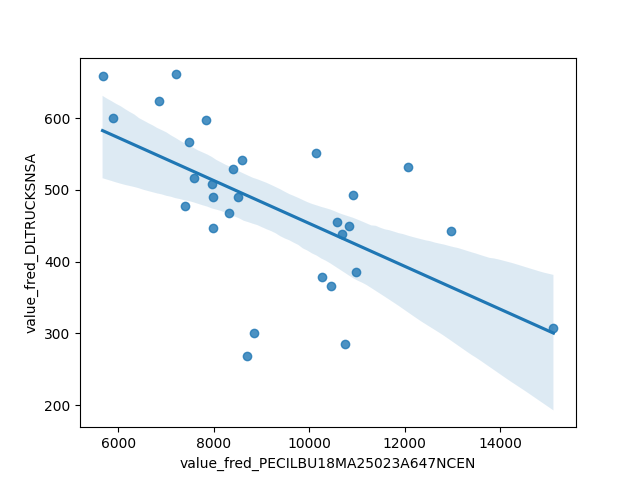
\includegraphics[scale = 0.9]{plots/plot_2024-09-28.png}
\caption{Regression Plot for 2024-09-28}
\end{figure}
\newpage


\include{tex_things/day_2024-09-29}

\end{document}
